\documentclass[./thesis.tex]{subfiles}

 \newcommand{\minDetInTeeth}{\text{minDetInTeeth}}
\newcommand{\Nteeth}{N_\text{teeth}}
\newcommand{\lTeethI}{\text{lTeethI}}

\begin{document}

\section{def}

\section{PT2 vs CIPSI}

CIPSI and PT2, all approximations aside, both imply computation of $\epsilon(\alpha)$ for all $\ket \alpha$, so both can be computed at the same time. CIPSI is about identifying the set of the largest ones, PT2 is about computing the sum over all of them. There are two main consequences to this
\paragraph{PT2 is one iteration behind CIPSI}
In a practical sense, CIPSI is ahead of PT2. A iteration $n$, identifiying the most significant $\ket \alpha$ is about building $\Psi^{n+1}$ while summing them is about estimating the cost of truncation for $\Psi^{n}$. Computing PT2 for a "final" wavefunction therefore requiers an extra iteration, which applies to a larger $\Psi$ and thus is more costly. ( autres implementation de PT2 possible ).

\paragraph{CIPSI can take more approximations}
Fully computing the sum has to be more costly than just identifying the greatest terms. As was said in SELECTION, the CIPSI algorithm can take pretty drastic approximations%, because we only try to identify the set of $\ket \alpha$ with the largest contributions $\epsilon(\alpha)$.
	\begin{itemize}
		\item{$t_g$}
		allows to explore a reduced subset of $\ket \alpha$ in which we are almost sure to find those of interest.
		\item{$t_s$}
		allows for a less accurate and less expensive computation of $\epsilon(\alpha)$, which is unlikely to significantly change the identified set.
	\end{itemize}
	These approximations do not apply when computing PT2. The very large number of smaller contributions makes them much harder to neglect. Unfortunately, increasing $t_g$ and $t_s$ thresholds dramatically increases the computational cost.


\paragraph{}

Unfortunately, a partial computation of PT2 results in a biased value. Since $\epsilon(\alpha)$ is an energy contribution, it's necessarily negative, and PT2 is a sum of same-sign contributions. Therefore, truncating it inevitably results in a bias, some energy is missing but there is little clue how much exactly. The $t_g$ and $t_s$ thresholds used in CIPSI can be seen as ways of minimizing this truncation's amplitude for a given computational cost.

Before the stochastic computation of PT2 was set up, our best choice was to set low $t_g$ and $t_s$ thresholds while performing CIPSI, and accept very approximated values for PT2 of intermediate wavefunctions ; then, once the selection was completed, we would highen them just for a final, very costly ``PT2 only'' iteration. In fact, an exact computation with $t_g=N_{gen}$ and $t_s=N_{det}$ was often prohibitively long, so the final PT2 was still biased. 

\section{Stochastic estimation of PT2}

We eventually solved the previously discussed problem by turning the bias into an error bar. The base idea is that, instead of trying to get the largest possible chunk of contribution, we can randomly pick $\epsilon(\alpha)$ contributions and make a Monte-Carlo estimate for the sum over all $\ket \alpha$. In this case, to avoid any bias we must set

\begin{equation}
t_g = N_{gen} ; t_s = N_{det}
\end{equation}


Not only the estimate will be unbiased and much closer to the actual PT2, but we will have an estimate for the error. Because PT2 is itself used as an approximation

\begin{equation}
E_{var} + E_{PT2} \simeq E_{fullCI}
\end{equation}

An error significantly smaller than the typical accuracy of $E_{var} + E_{PT2}$ VS $E_{fullCI}$ is certainly acceptable.


For different reasons, the actual Monte-Carlo computation is significantly more convoluted than simply drawing random $\ket \alpha$. 

\paragraph{$\epsilon(\alpha)$ are packed into elementary contributions $e_I$}
Individual $\epsilon(\alpha)$ are expensive to compute. In the CIPSI algorithm, each generator determinant creates a number of unique $\alpha$, and computes $\epsilon(\alpha)$ for each one of them.
Essentially, $\ket \alpha$ are grouped in $N_{gen}$ disjoint sets, each associated with a generator determinant, as shown in figure \ref{fig:mu_sample}.

\begin{equation}
\epsilon(\alpha) \in \mathcal{A}_i ; \Hij{\alpha}{\Psi_i} \neq 0 ; \Hij{\alpha}{\Psi_{j<i}} =0 
\end{equation}

Because of the numerous tricks used, we could compute all $\epsilon(\alpha)$ from one set considerably faster than if we had to compute each one separately. Therefore, in order to access a larger chunk of data, the stochastic PT2 algorithm will not consider individual $\epsilon(\alpha)$, but instead sums of all $\epsilon(\alpha)$ from the same set.
The elementary contributions we are considering, aren't $\epsilon(\alpha)$, but
\begin{equation}
e_I = \sum_{\alpha \in \mathcal{A}_I} \epsilon(\alpha)
\end{equation}
Indeed
\begin{equation}
E_{PT2} = \sum_{I} e_I
\end{equation}

$e_I$ are already explicitely computed by our CIPSI implementation, which returned the aggregated values of $\epsilon(\alpha)$ for one job, one job being essentially a generator determinant.

\paragraph{$e_I$ can be stored to avoid re-computation}
Each elementary contribution is associated with a generator determinant, so there are only $N_{gen}$ elementary contributions. This is small enough so, when a $e_I$ contribution is computed, its value can be stored and simply re-used if the same sample is drawn again. This, in turn, means the exact result will eventually be known once every sample has been computed. The cost for this will essentially be the same as that of the purely deterministic, full computation, with a negligible additional cost due to the Monte-Carlo related computations ( drawing random numbers, finding the associated samples... ).

\section{Monte-Carlo sampling}

We generally want to estimate the value of a sum over $N$ samples $s_i$
\begin{equation}
S = \sum_{i=1}^N {s_i}
\end{equation}

After randomly drawing $n$ sample indices (the same one can be drawn several times) forming the set $\{\mathcal{S}\}$, we can estimate $S$ as

\begin{equation}
\tilde S = \frac{N}{n} \sum_{i \in \{\mathcal{S}\}} {s_i}
\end{equation}

with an estimated error (A VERIFIER XXXXXXXXXXXXXXXXXXXXXXXXXXXXXXXX)

\begin{equation}
\sqrt{ \Big ((\sum_{i \in \{\mathcal{S}\}} {s_i})^2 - \sum_{i \in \{\mathcal{S}\}} {s^2_i} \Big )n^{-1} }
\end{equation}

The greatest the variance of $s_i$, the slowest the convergence. It is common to use a probability distribution $w$ as a convergence accelerator. We rewrite $S$ as 

\begin{equation}
S = \sum_{i=1}^N {w_i \times \frac{s_i}{w_i}}
\end{equation}

which can be estimated by drawing sample indices $i$ with a probability of $w_i$ forming the set $\{\mathcal{S'}\}$, the associated sample values being $\frac{s_i}{w_i}$

\begin{equation}
\tilde S' = \frac{1} {\sum_{i \in \{ \mathcal{S'} \} } w_i} \sum_{i \in \{\mathcal{S'}\}} {s_i}
\end{equation}

Not using a repartition function is the particular case of drawing $\frac{s_i}{1}$ with a uniform probability ($1$ normalized over the $N$ samples). The variance of this sample space is that of $\frac{s_i}{w_i}$ rather than $s_i$. An ideal repartition function $w^\star$ would be so that

\begin{equation}
\frac{s_i}{w^\star_i} = K
\end{equation}

with $K$ any constant. The variance would be zero, so covergence would be reached after a single sample is drawn. Even an extremely rough approximation of $w^\star$ will improve convergence.



The representation we are going to use is a horizontal serie of $N$ boxes of width $w_i$, containing the sample index $i$.
The sample index $i$ associated with drawing a random number $u \in [0,1)_\mathbb{R}$ is noted $w[u]$. It is determined using the cumulative repartition function $W$
\begin{align}
W_j = \sum_{k \leq j} w_k \\
W_{i-1} \leq u < W_i
\end{align}

\begin{figure}[h!]
	\begin{center}
		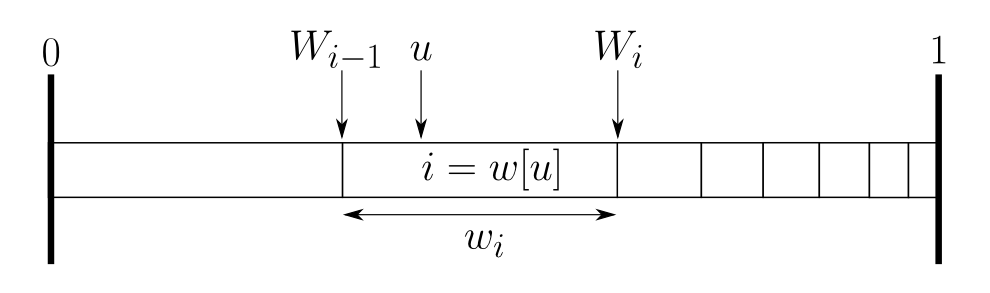
\includegraphics[width=0.9\columnwidth]{figures/pt2/mc_representation}
		\caption{Schematic representation of a Monte-Carlo computation}
		\label{fig:mc_representation}
		Drawing the random number $u$ with the repartition function $w$ yields sample index $i=w[u] = 2$
	\end{center}
\end{figure}





\section{The sample space}

\paragraph{``Sample'' and ``Comb''}
Because of its original nature, this algorithm casts some ambiguity on what should be refered to as a ``sample''. We are going to estimate a sum of elementary contributions $e_I$, compute and store them individually, and draw them based on a repartition function ; therefore they will be refered to as the \emph{samples} and shown as such in the previously introduced representation. But the values actually treated as samples in the statistical sense ($s_i$ in the previous section), are sums over several $e_I$, refered to as \emph{combs}.


\paragraph{$C_I^2$ is used as a repartition function}
Generator determinants are sorted with decreasing absolute values of $C_I$.
	As can be seen in figure \ref{fig:ei}, the values of $e_I$ span many orders of magnitude and decrease rapidly with $I$, in an exponential-looking way. Smoothed values for $e_I$ are shown in figure \ref{fig:p_i}. There are a few reasons for that.
\begin{itemize}
	\item
	The values for the denominator $\Delta E_\alpha$ used in the computation of $\epsilon(\alpha)$ tend to increase, as variational determinants tend to be more and more excited and to populate higher orbitals ( detailler ? )
	\item
	The number of unique $\ket \alpha$ per generator decreases. Indeed, the more ``previous generators'' there is, the likelier it is that a generated $\ket \alpha$ was generated before.
	\item
	Unique $\ket \alpha$ are, by construction, disconnected from all previous generators, which mean they connect to a smaller and smaller norm of $\Psi$ ( see figure \ref{fig:a_con} ). 
\end{itemize}


The last reason given for the decrease of $e_I$ is the most important one, and tells us that the most significant $\alpha$ are those connecting to $\kI$, so the dominant terms of $e_I$ are 

\begin{equation}
\frac{C_I^2 \Hij{I}{\alpha}\Hij{\alpha}{I}}{\Delta E_{\alpha}}
\end{equation}

Consequently we chose

\begin{equation}
\tilde w_I = C_I^2
\end{equation}

as a repartition function for $e_I$. This is however not the exact repartition function used in the Monte-Carlo scheme. We will later introduce some slight modification to it, for algorithmic reasons.
As can be seen in figure \ref{fig:eici2}, $\frac{e_I}{C_I^2}$, which is very close to our sample space, indeed has a lower variance than $e_I$ but is still similar in that it spans orders of magnitude and overall decreases.

\paragraph{Hybrid deterministic-stochastic aspect}
Because $e_I$ decreases rapidly, most of the contribution is contained in the first samples. We can entierely compute the first samples, and only make a stochastic estimation for the sum of the smaller ones. This effectively splits the sample space in two ranges, a deterministic one, then a stochastic one (hence the hybrid characteristic of this method), and our estimated energy

\begin{equation}
E_{PT2} = E_D + E_S
\end{equation}

with $E_D$ the exact energy for the deterministic part, and $E_S$ the estimated energy of the stochastic part. The error bar only applies to $E_S$, which is a fraction of the whole sum.
We call $n_0$ the number of samples in this deterministic part and $u_0 = W_{n_0}$ its weight.



\paragraph{The sample space is divided in $N_{teeth}$ \emph{teeth}}

Because $\frac{e_I}{C_I^2}$ overall decreases, it follows that small ranges have a lower variance than the whole set. The entire space of $\frac{e_I}{C_I^2}$ is split in $N_{teeth}$ ranges refered to as \emph{teeth}. In figure \ref{fig:eici2comb}, the space of stochastic $\frac{e_I}{C_I^2}$ has been split in \alert{five teeth $P_1$ to $P_4$}. The variance inside each tooth is expected to be, quite clearly, much smaller than the variance for the whole space.

Therefore, instead of drawing individual indices, we are going to draw ``combs'' of indices, which are correlated sets of 1 index from each tooth ; the associated sample value is the sum of $e_I$ over those indices. Intuitively, the sum of ``one large, one medium and one small'' has a lower variance than the sum of ``three at random''.

We are sampling combs, but we have defined a repartition function for $e_I$. Since we impose that the same number of $e_I$ are drawn in each tooth - one per comb - we effectively give all teeth the same weight $W_T=\frac{1-u_0}{N_{teeth}}$ in the Monte-Carlo scheme. Therefore, the actual weight given to $e_I \in P_x$ is

\begin{equation}
w_I = W_T \times \frac{\tilde w_I}{\sum_{J \in P_x} \tilde w_J}
\end{equation}

To leave the repartition function unaltered, we need all teeth to actually weight $W_T$

\begin{equation}
\sum_{J \in P_x} \tilde w_J = W_T
\end{equation}

Clearly this is not acheivable for any reartition function $\tilde w$. Schematically, it would require the threshold between two teeth to exactly match the threshold between two $e_I$. It is possible to artificially split a $e_I$ to get a matching threshold, but this adds some complexity algorithmically speaking.

We will later enforce that all teeth contain at least 5-10 samples - and often a lot more, up to hundreds of thousands. Therefore, a simpler solution is to ``round'' the teeth thresholds to the $e_I$ threshold directly above, which will result in teeth with weights close to $W_T$, and thus the actual repartition function will be little different from the one we initially defined. Since our repartition function is an extremely rough estimation of $e_I$, to say the least, it is unlikely to cause any significant change in convergence speed.
Essentially, we will use $\tilde w$ only to define which sample goes in which tooth, then use $w$ as the actual repartition function. This gives us, by definition, teeth weighting exactly $W_T$.

We can now define $B(u)$ the value of the comb associated with drawing $u \in [0,1)_\mathbb{R}$

\begin{equation}
B(u) = \sum_{i=0}^{N_{teeth}-1} e_{w[u_0+ W_T(u+i)]}
\end{equation}

\paragraph{fully-computed teeth are moved to the ``deterministic'' part}
%The deterministic part could in principle extend to the first $e_{I \in P_n}$ whose value is unknown, exclusive. This however is algorithmically complex because some combs 
Given the first $e_{I \in P_t}$ whose value is unknown, we extend the deterministic range to $P_t$, exclusive. This implies $t$ is a parameter of $n_0$ and $u_0$

\begin{equation}
n_0 = n_0(t) = \lTeethI[t]-1
\end{equation}
\begin{equation}
u_0 = u_0(t) = W_{n_0(t) -1}
\end{equation}

It also implies all teeth $P_{n<t}$ must be ignored in combs, as they are not part of the stochastic range. We have to make $t$, the index of the first non-deterministic tooth, a parameter of comb values

\begin{equation}
B_t(u) = \sum_{i=0}^{N_{teeth}-t} e_{w[u_0(t)+ W_T(u+i)]}
\end{equation}
%B_t(u) = \sum_{i=t}^{N_{teeth}} e[u_0+ W_{teeth}(u+i-1)]

To be able to compute average and standard error 

\begin{align}
 S_t = \sum_{u \in {U}} B_t(u) \\
 S^2_t = \sum_{u \in {U}} B_t(u)^2
\end{align}


\section{Practical considerations}

There are a few more practical details that must be dealt with.

\subsection*{initial deterministic part}

For each comb, we draw a sample $e_I$ in each teeth. When a tooth is entirely computed, it is moved to the deterministic part. Thus, it is immediately obvious that a tooth containing a single sample makes no sense, as it will be instantly moved to the deterministic part ; it can as well be considered part of it. Because it's usually accepted (???) that it takes at least 30 samples to estimate a variance, we can go further and consider that a tooth with fewer than 5-10 samples will be moved to the deterministic part too fast to be of real interest.
%Because samples are sorted with decreasing $w_i$, each tooth is guaranteed to contain as many or more samples than the previous one,  therefore we only need to ensure the first tooth contains at least 5-10 samples.
%In fact because of the "tooth filling" mechanism described later on, we know the first tooth has to contain at least 31 samples to ever be non-deterministic. 


\subsection*{tooth filling}

This is an empirical mechanism to balance the stochastic and deterministic aspect of this method. For a tooth containing $n$ samples of equal weight, full computation is acheived after on average (A VERIFXXXXXXXXXXXXXXXXXXXXXXX)

\begin{equation}
\sum_{i=0}^{n-1} \frac{n}{n-i}
\end{equation}

combs are drawn. Thus, teeth containing thousands of determinants are very hard to move to the deterministic part. A tooth containing 10000 samples with a single uncomputed one, only needs computation of a single sample to be moved to the deterministic part, but one has to wait on average 10000 more combs are drawn until by chance the right sample is computed.
A convenient way to avoid this frustrating situation is, everytime a comb is drawn, to additionally compute the first uncomputed sample of the whole space. This ensures smooth filling of teeth, and that that the full deterministic computation will be achieved before $N_{gen}$ combs are drawn.

\section{implementation}



\subsection{drawing}

The algorithm to find a sample index associated with drawing $u$ in with a repartition function $w$ is show as algorithm \ref{alg:FIND_SAMPLE}.

\begin{algorithm}
\label{alg:FIND_SAMPLE}
\caption{FIND\_SAMPLE}
\SetKwFunction{FFind}{FIND\_SAMPLE}
	\SetKwProg{Fn}{Function}{:}{}
	
	\Fn(\tcc*[h]{Finds sample index associated with drawing random value $v$ in a cumulative probability distribution $p$}){\FFind{$v$,$p$}}{
		\KwData{$0 \leq v < 1$}
		%\KwData{$cw[l-1] \leq v < cw[r] ; cw[0] = 0$}
		\KwResult{Returns $i$ so that $p[i-1] \leq v < p[i]$. It's implied $p[0] = 0$}
		\tcc {The result must be in the range $[l,r]$. We set them for the most general case}
		$l \gets 1$ \;
		$r \gets \text{size of array } p$ \;
		
		\uIf{$v < p[l]$}{
			\KwRet $l$ \;
		}\ElseIf{$l-r \leq 1$}{
			\KwRet $r$ \;
		}
		\While{$r-l > 1$}{
			$i \gets \lfloor (r-l) / 2 \rfloor$ \;
			\uIf{$p[i] < v$}{
				$l \gets i$ \;
			}
			\Else{
				$r \gets i$ \;
			}
		}
		\KwRet $r$ \;
	}
\end{algorithm}




\subsection{building teeth}

\begin{itemize}

\item
\emph{input}
\begin{description}
\item[$\tilde w$]
The initial repartition function, which we chose to be $C_I^2$.
\item[$\Nteeth$]
A desired number of teeth
\item[$\minDetInTeeth$]
A desired minimal number of samples per teeth
\end{description}

\item
\emph{output}
\begin{description}
\item[$w$]
The repartition function
\item[$\lTeethI, $]
An array of size $\Nteeth$, with $\Nteeth[i+1]$ being the index of the first sample of teeth $P_i$. For algorithmic convenience, $\lTeethI[\Nteeth+1] = \Ndet+1$  
\end{description}
\end{itemize}


There is no trivial way to ensure teeth building will succeed with a given set of parameters. 
With $n_0$ the size of the initial deterministic set, teeth building is sure to fail if 
\begin{equation}
N_{det} - n_0 < \minDetInTeeth \times \Nteeth
\end{equation}
However, it may not succeed as there is no guarantee the first tooth will contain $\minDetInTeeth$ samples. Because samples are sorted with decreasing $\tilde w_I$, each tooth is guaranteed to contains as many or more samples than the previous one.
Relying on the fact that $\tilde w_i$ get more and more balanced, we increment $n_0$ until either the first tooth contains enough samples, or the impossibility condition is reached.

\begin{algorithm}
	$\tilde W_I = \sum_{i \leq I} {\tilde w_i}$ \;
	$n_0 \gets 0$ \;
	$l \gets 0$ \;
	$r \gets \tilde W[\minDetInTeeth]$ \;	
	\While{}{
		$\text{teeth\_width} = \frac{1 - l}{N_{teeth}}$ \;
		\If{$\text{teeth\_width} < r - l$}{
			break \;
		}
		
		$s \gets s + 1$ \;
		\If{$N_{det} - n_0 < \minDetInTeeth \times \Nteeth$}{
			STOP cannot compute with those parameters \;
		}
		$r \gets \tilde W[n_0+\minDetInTeeth]$ \;
		$l \gets \tilde W[n_0]$\;
	}
	%$\lTeethI[1] = s+1$ \;
\end{algorithm}

Then, $\lTeethI$ can be fully computed

\begin{algorithm}
	\caption{COMPUTE\_TEETH}
	$\lTeethI[1] = s+1$ \;
	\For{$t=2,N_{teeth}$}{
		$r = l + teeth\_width \times t$ \;
		$\lTeethI[t] = FIND\_SAMPLE(r, \tilde W)$ \;
	}
	$\lTeethI[\Nteeth+1] = \Ndet+1$ \;
\end{algorithm}

And the actual repartition function $w$

\begin{algorithm}
	\caption{COMPUTE\_TEETH}
	
	\For{$t=1,N_{teeth}$}{
		$\text{tooth\_width} = \tilde W_{\lTeethI[t+1]-1} - \tilde W_{\lTeethI[t]-1}$ \;
		\For{$i=\lTeethI[t], \lTeethI[t+1]-1$}{
		$w_{i} = \tilde w_{i} \times (\Nteeth \times \text{tooth\_width})^{-1}$ \;
		}
	}
	
\end{algorithm}



\subsection{building job queue}

For a massively parallel implementation, we need to create a job queue. Because values for $e_I$ are stored, quite clearly, we need 1 job per generator determinant. Because of the tooth filling mechanism, we know we will need at most $N_{gen}$ combs.


\begin{algorithm}
	$M \gets $ array size $N_{gen}$ initialized to 0 \;
	$N_c \gets 0$ \;
	$F \gets 0$ \;
	$N_j \gets n_0(1)$ \;
	
	\For{$i=1,n_0(1)$}{
		$d_i \gets TRUE$ \;
		$J_i \gets i$ \;
	}
	
	\For{$i=1,N_{gen}$}{
		$comb[i] \gets $ random value in $[0,1)_\mathbb{R}$ \;	
	}
	
	\While{$N_j < N_{gen}$}{
		$N_c \gets N_c + 1$ \;
  		\For{$t=0,N_{teeth}-1$}{
		%$v \gets lTeeth[t] + rand \times toothSize[t]$ \;
		$v \gets u_0(t) + comb[N_c] \times W_T$ \;
		
		%$i=FIND\_SAMPLE(rand, lTeethI[t], rTeethI[t])$ \;
		$i=FIND\_SAMPLE(v, W)$ \;
		\If{$not\ d_i$}{
			$N_j \gets N_j + 1$ \;
			$J_{N_j} \gets i$ \;
			$d_i \gets TRUE$ \;
		}
	}
	$M_{N_j} \gets N_c$ \;
   \While{$F < N_{gen}$}{
    	$F \gets F + 1$ \;
        \If{$not\ d_F$}{
          $d_F \gets TRUE$ \;
           $N_j \gets N_j+1$ \;
           $J_{N_j} \gets F$ \;
           break \;
         }
	  }
	}
	
\end{algorithm}

\subsection{computing estimation and error}


\begin{algorithm}
	$n \gets 1$ \;
	$t \gets 1$ \;	
	\While{$n \leq N_{gen}$}{
		retrieve $I$ and $e_I$ \;
		store $e_I$ \;
		$d_I \gets TRUE$ \;
		\While{$n \leq N_{gen}$}{
			\If{$d_n$}{
				\If{$n \geq n_0(t)$}{
					$t \gets t+1$ \;
				}
				\If{$M[n] \neq 0$}{
					$S_* \gets S_* + B_*(comb[M[n]])$ \;
					$S^{(2)}_* \gets S^{(2)}_* + B_*(comb[M[n]])^2$ \;				
				}
			}
			$n \gets n+1$ \;
		}
		\tcc{\alert{A VERIFIERXXXXXXXXXXXXXXXXXXXXXXXX}}
		error $\gets \sqrt{(S_t^2 - S^{(0)}_t) n^{-1} }$
		return on whatever condition \;
	}
	\tcc{full computation done}
\end{algorithm}

\begin{algorithm}
	\tcc{efficiently computes $S_* \gets S_* + B_*(u)$  and $S^{(2)}_* \gets S^{(2)}_* + B_*(u)^2$}
	
					
	$x \gets 0$ \;
	\For{$t=N_{teeth},1,-1$}{
		$I \gets FIND\_SAMPLE(u_0(t)+u \times W_T, W)$ \;
		$x \gets x + e_{I}$ \;
		$S_t \gets S_t + x$ \;
		$S^{(2)}_t \gets S^{(2)}_t + x^{2}$ \;
	}
\end{algorithm}



\begin{figure}[h!]
	\begin{center}
		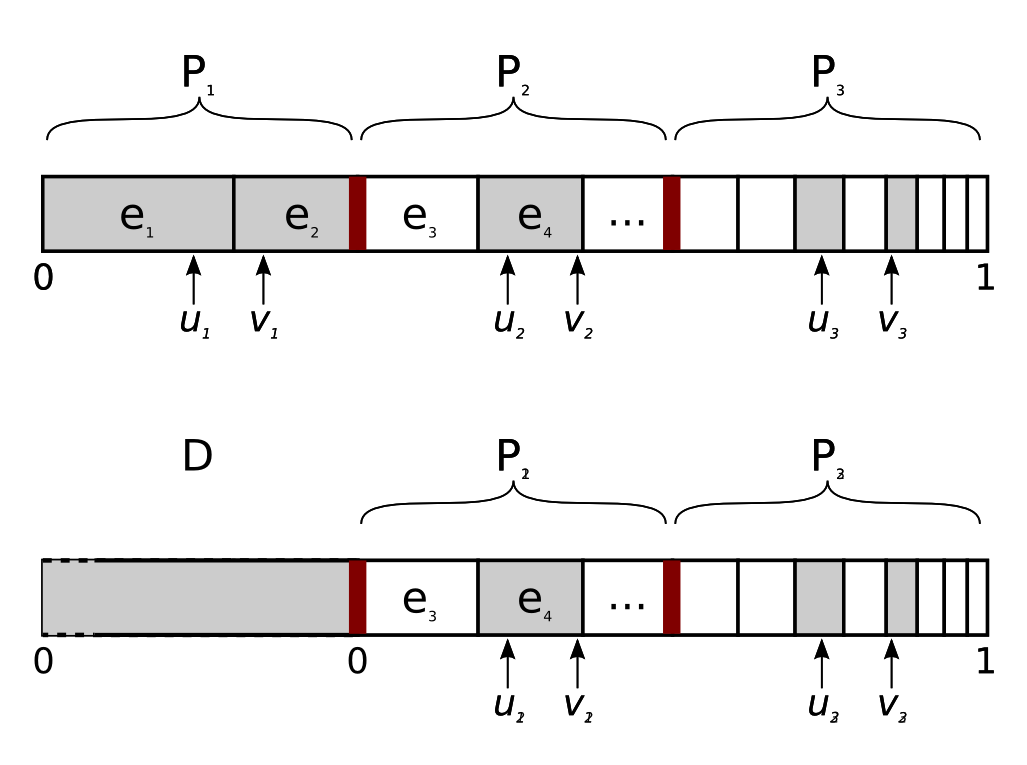
\includegraphics[width=0.9\columnwidth]{figures/pt2/move_to_deterministic}
		\caption{A REFAIRE NOTATION.............}
		\label{fig:move_to_deterministic}
		$e_I$
	\end{center}
\end{figure}

\begin{figure}[h!]
	\begin{center}
		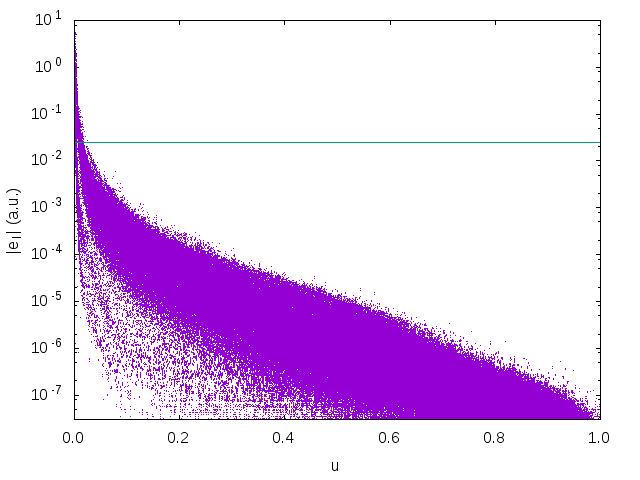
\includegraphics[width=0.9\columnwidth]{figures/pt2/eI}
		\caption{A REFAIRE NOTATION.............}
		\label{fig:ei}
		$e_I$
	\end{center}
\end{figure}

\begin{figure}[h!]
	\begin{center}
		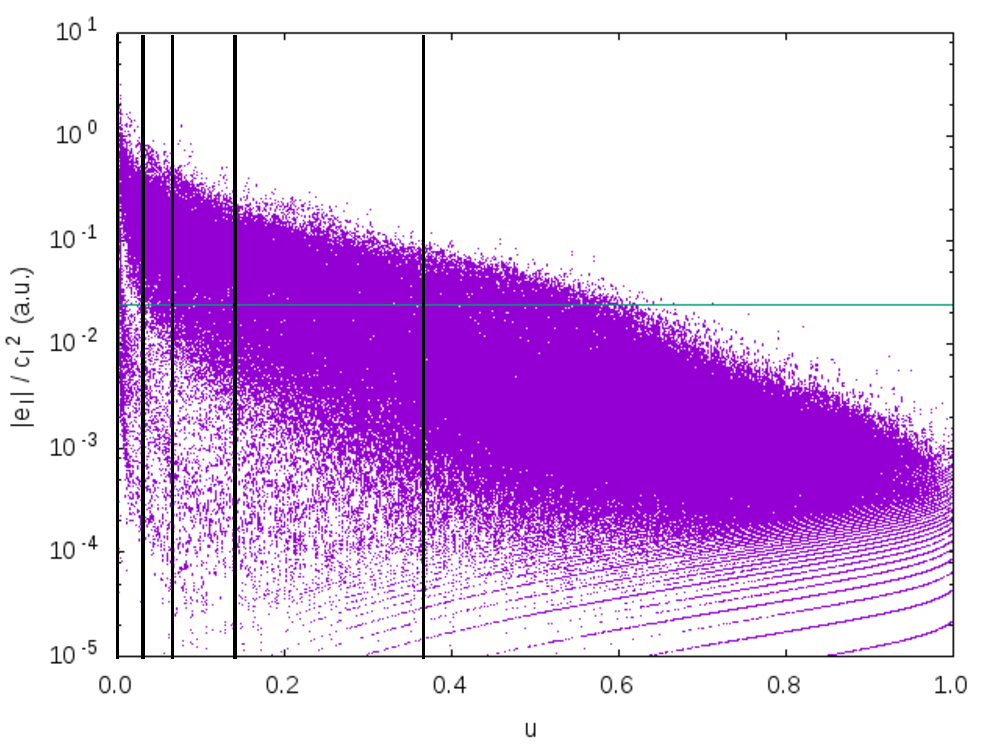
\includegraphics[width=0.9\columnwidth]{figures/pt2/eici2comb}
		\caption{A REFAIRE NOTATION.............}
		\label{fig:eici2comb}
		$e_I$
	\end{center}
\end{figure}

\begin{figure}[h!]
	\begin{center}
		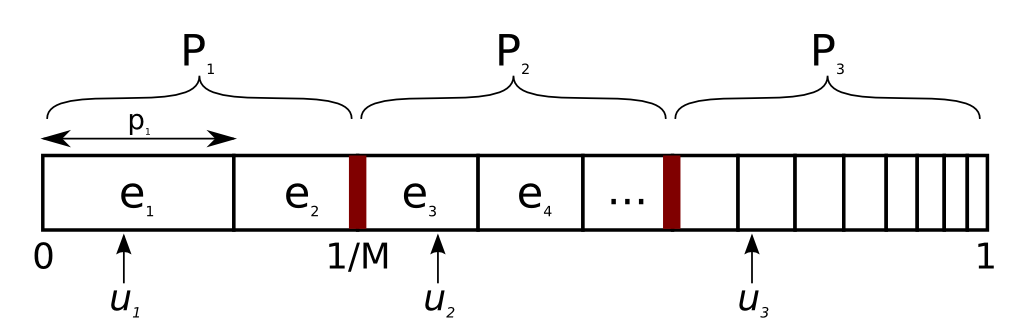
\includegraphics[width=0.9\columnwidth]{figures/pt2/comb}
		\caption{A REFAIRE NOTATION.............}
		\label{fig:comb}
		$e_I$
	\end{center}
\end{figure}


\begin{figure}[h!]
	\begin{center}
		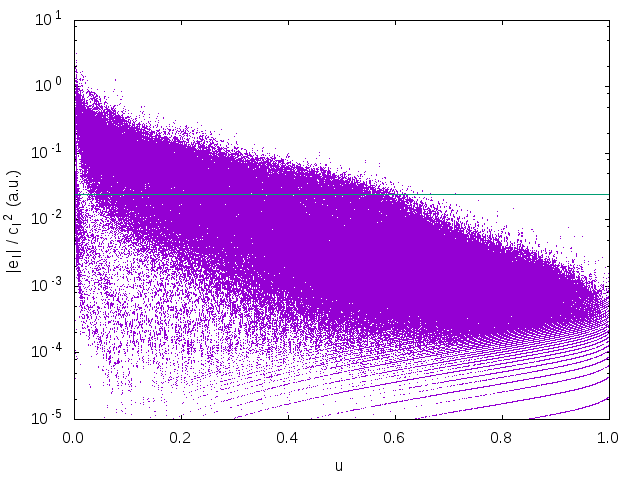
\includegraphics[width=0.9\columnwidth]{figures/pt2/eici2}
		\caption{A REFAIRE NOTATION.............}
		\label{fig:eici2}
		$e_I$
	\end{center}
\end{figure}


\begin{figure}[h!]
	\begin{center}
		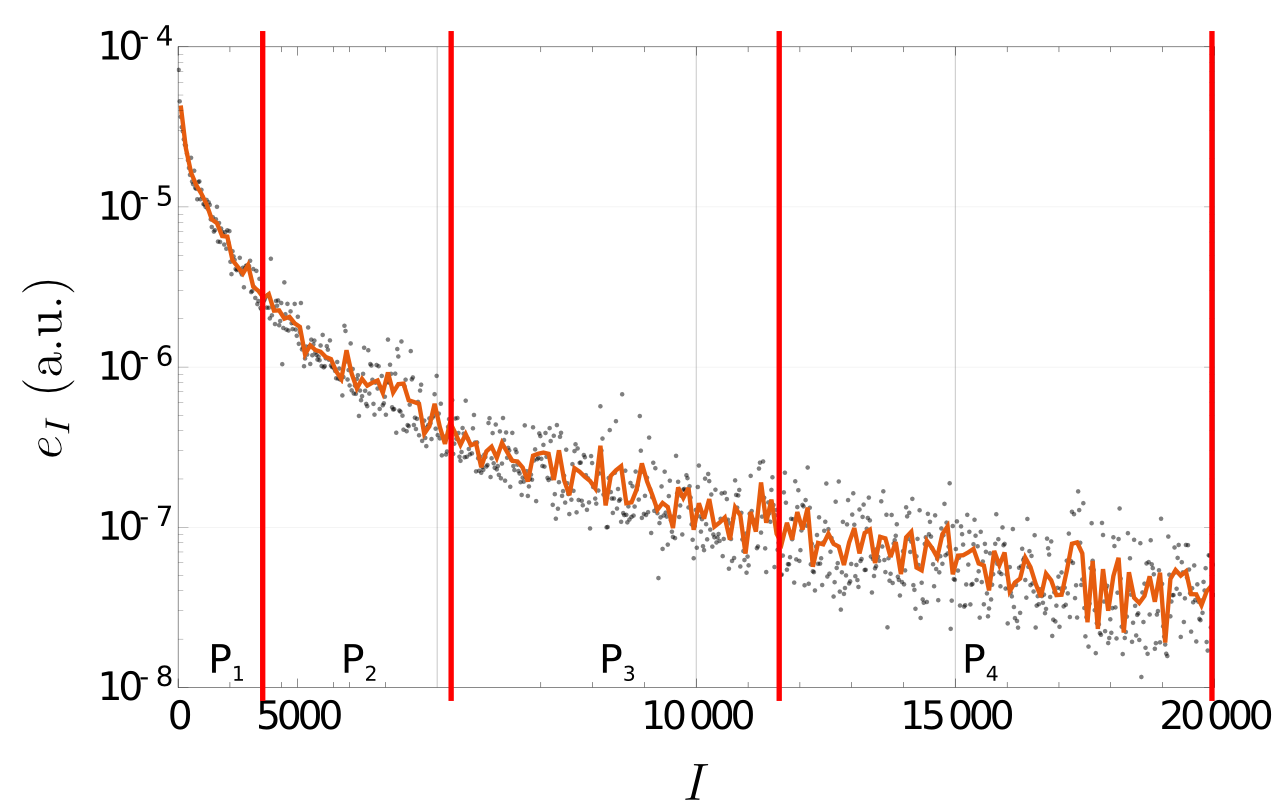
\includegraphics[width=0.9\columnwidth]{figures/pt2/P_i}
		\caption{A REFAIRE NOTATION.............}
		\label{fig:p_i}
		$e_I$
	\end{center}
\end{figure}


\begin{figure}[h!]
	\begin{center}
		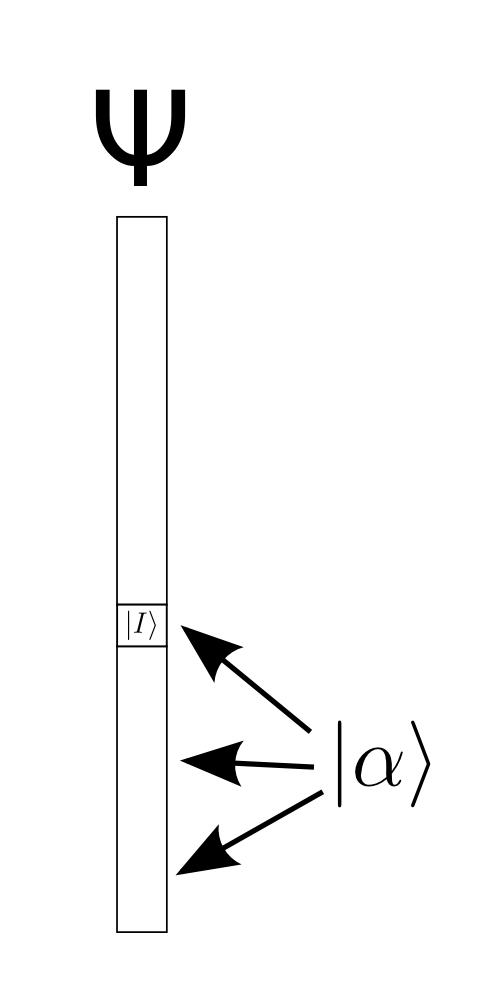
\includegraphics[width=0.2\columnwidth]{figures/pt2/a_con}
		\caption{A REFAIRE NOTATION.............}
		\label{fig:a_con}
		$\ket \alpha$ generated by increasing $\Psi_i$ connect to smaller and smaller norm of $\Psi$.
	\end{center}
\end{figure}

\begin{figure}[h!]
	\begin{center}
		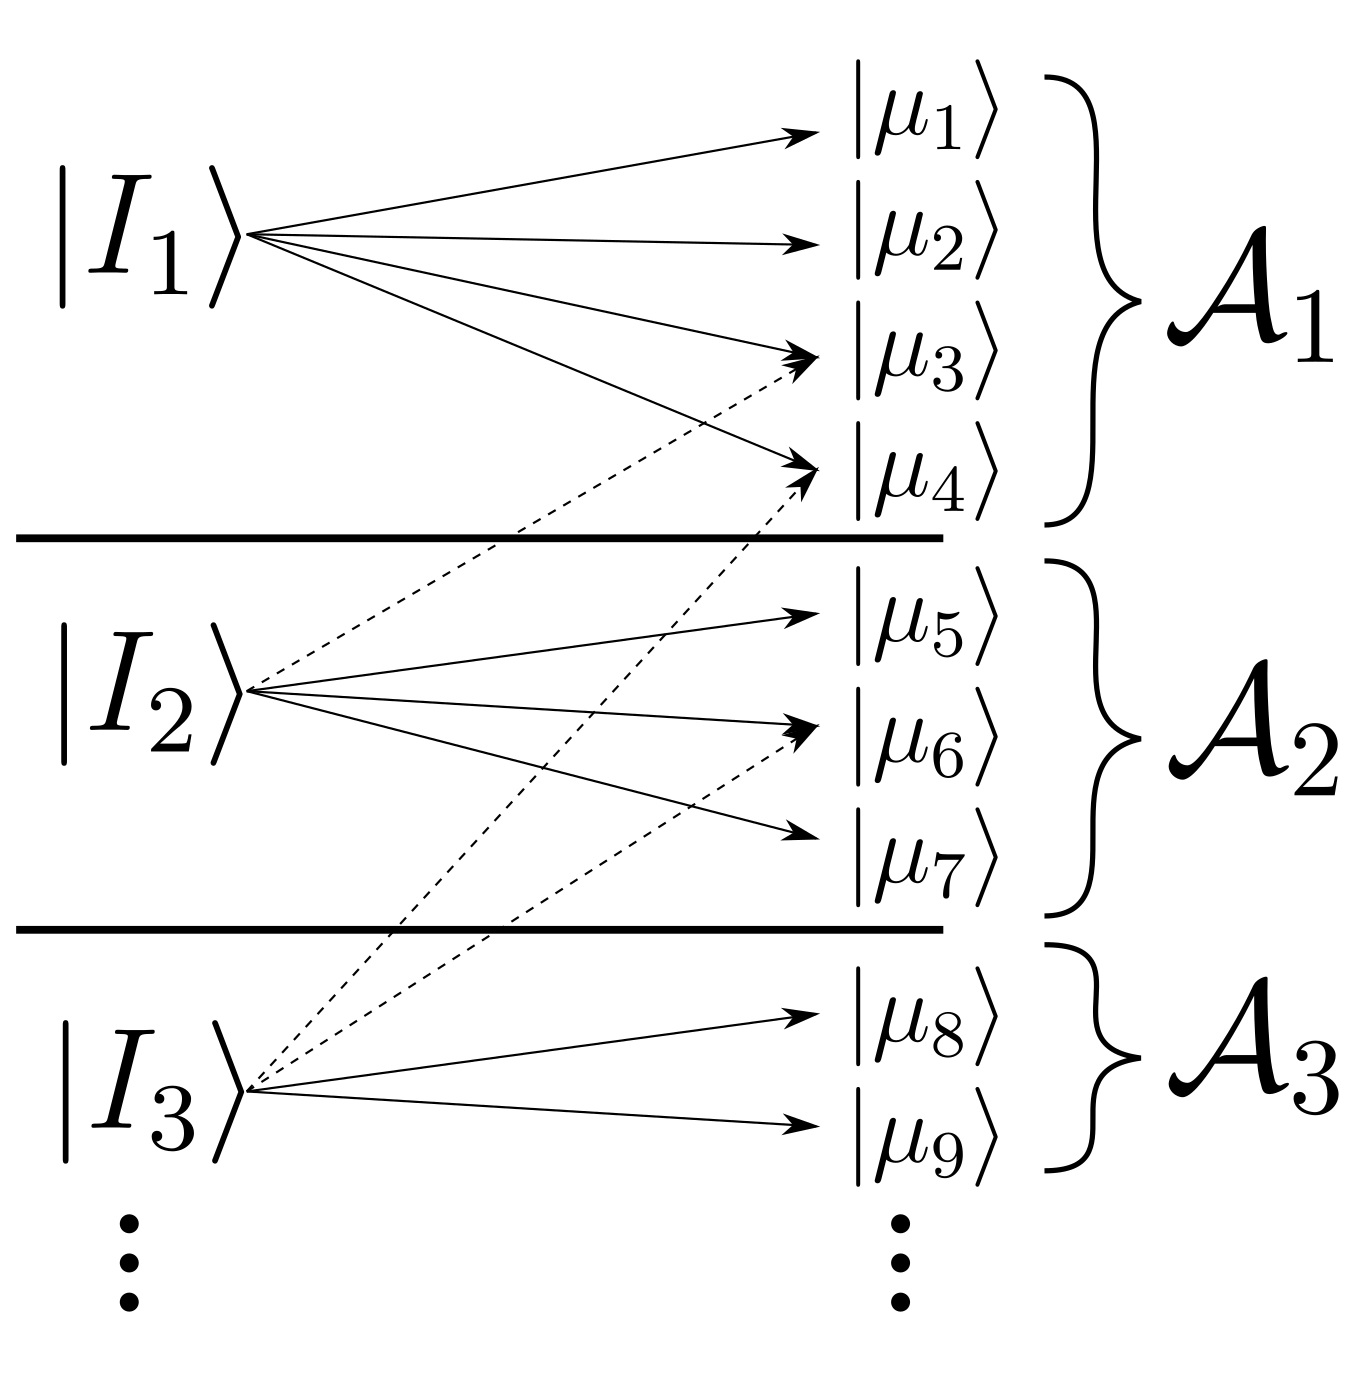
\includegraphics[width=0.5\columnwidth]{figures/pt2/mu_sample}
		\caption{}
		\label{fig:mu_sample}
		Construction of batches of $\ket \alpha$
	\end{center}
\end{figure}



\begin{figure}[h!]
	\label{comb_variables}
	\begin{center}
		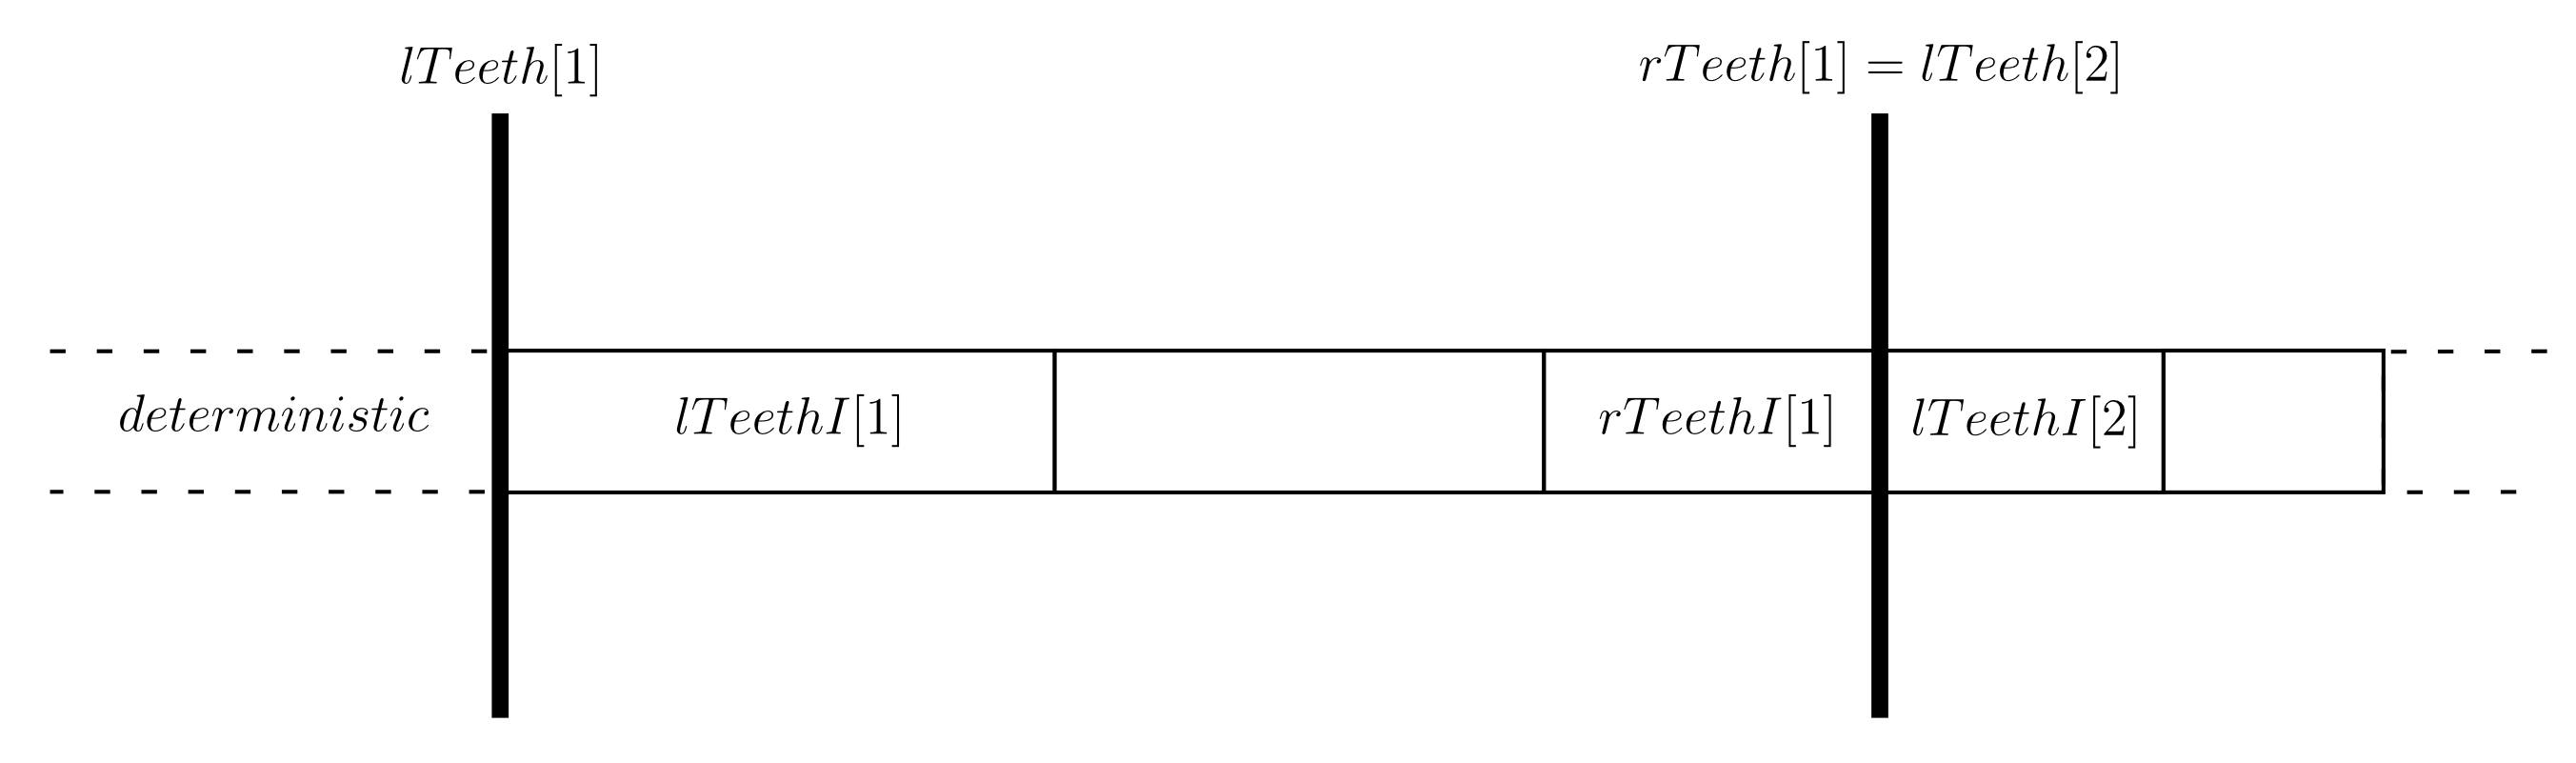
\includegraphics[width=1.00\columnwidth]{figures/pt2/teeth}
		\caption{comb}
		Variable names for the "comb" partition of $\Psi$. In boxes are shown indices, above are shown probabilities
		
\begin{equation}
toothOfDet[i] = t ; i \in \big [ lTeethI[t],rTeethI[t] \big ]
\end{equation}

		
\begin{equation}
toothSize[t] = rTeeth[t] - lTeeth[t]
\end{equation}

	\end{center}
\end{figure}

\begin{figure}[h!]
	\begin{center}
		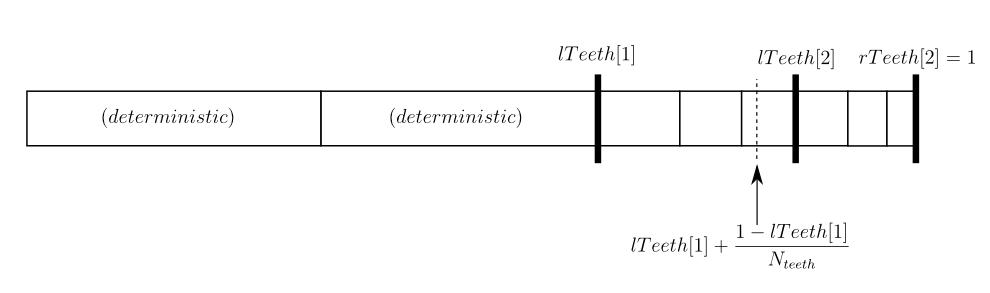
\includegraphics[width=1.00\columnwidth]{figures/pt2/teeths}
		\caption{\label{filtering}}
		Construction of teeth with $N_{teeth} = 2$ and 2 samples in the initial deterministic set.
	\end{center}
\end{figure}

\begin{figure}[h!]
	\begin{center}
		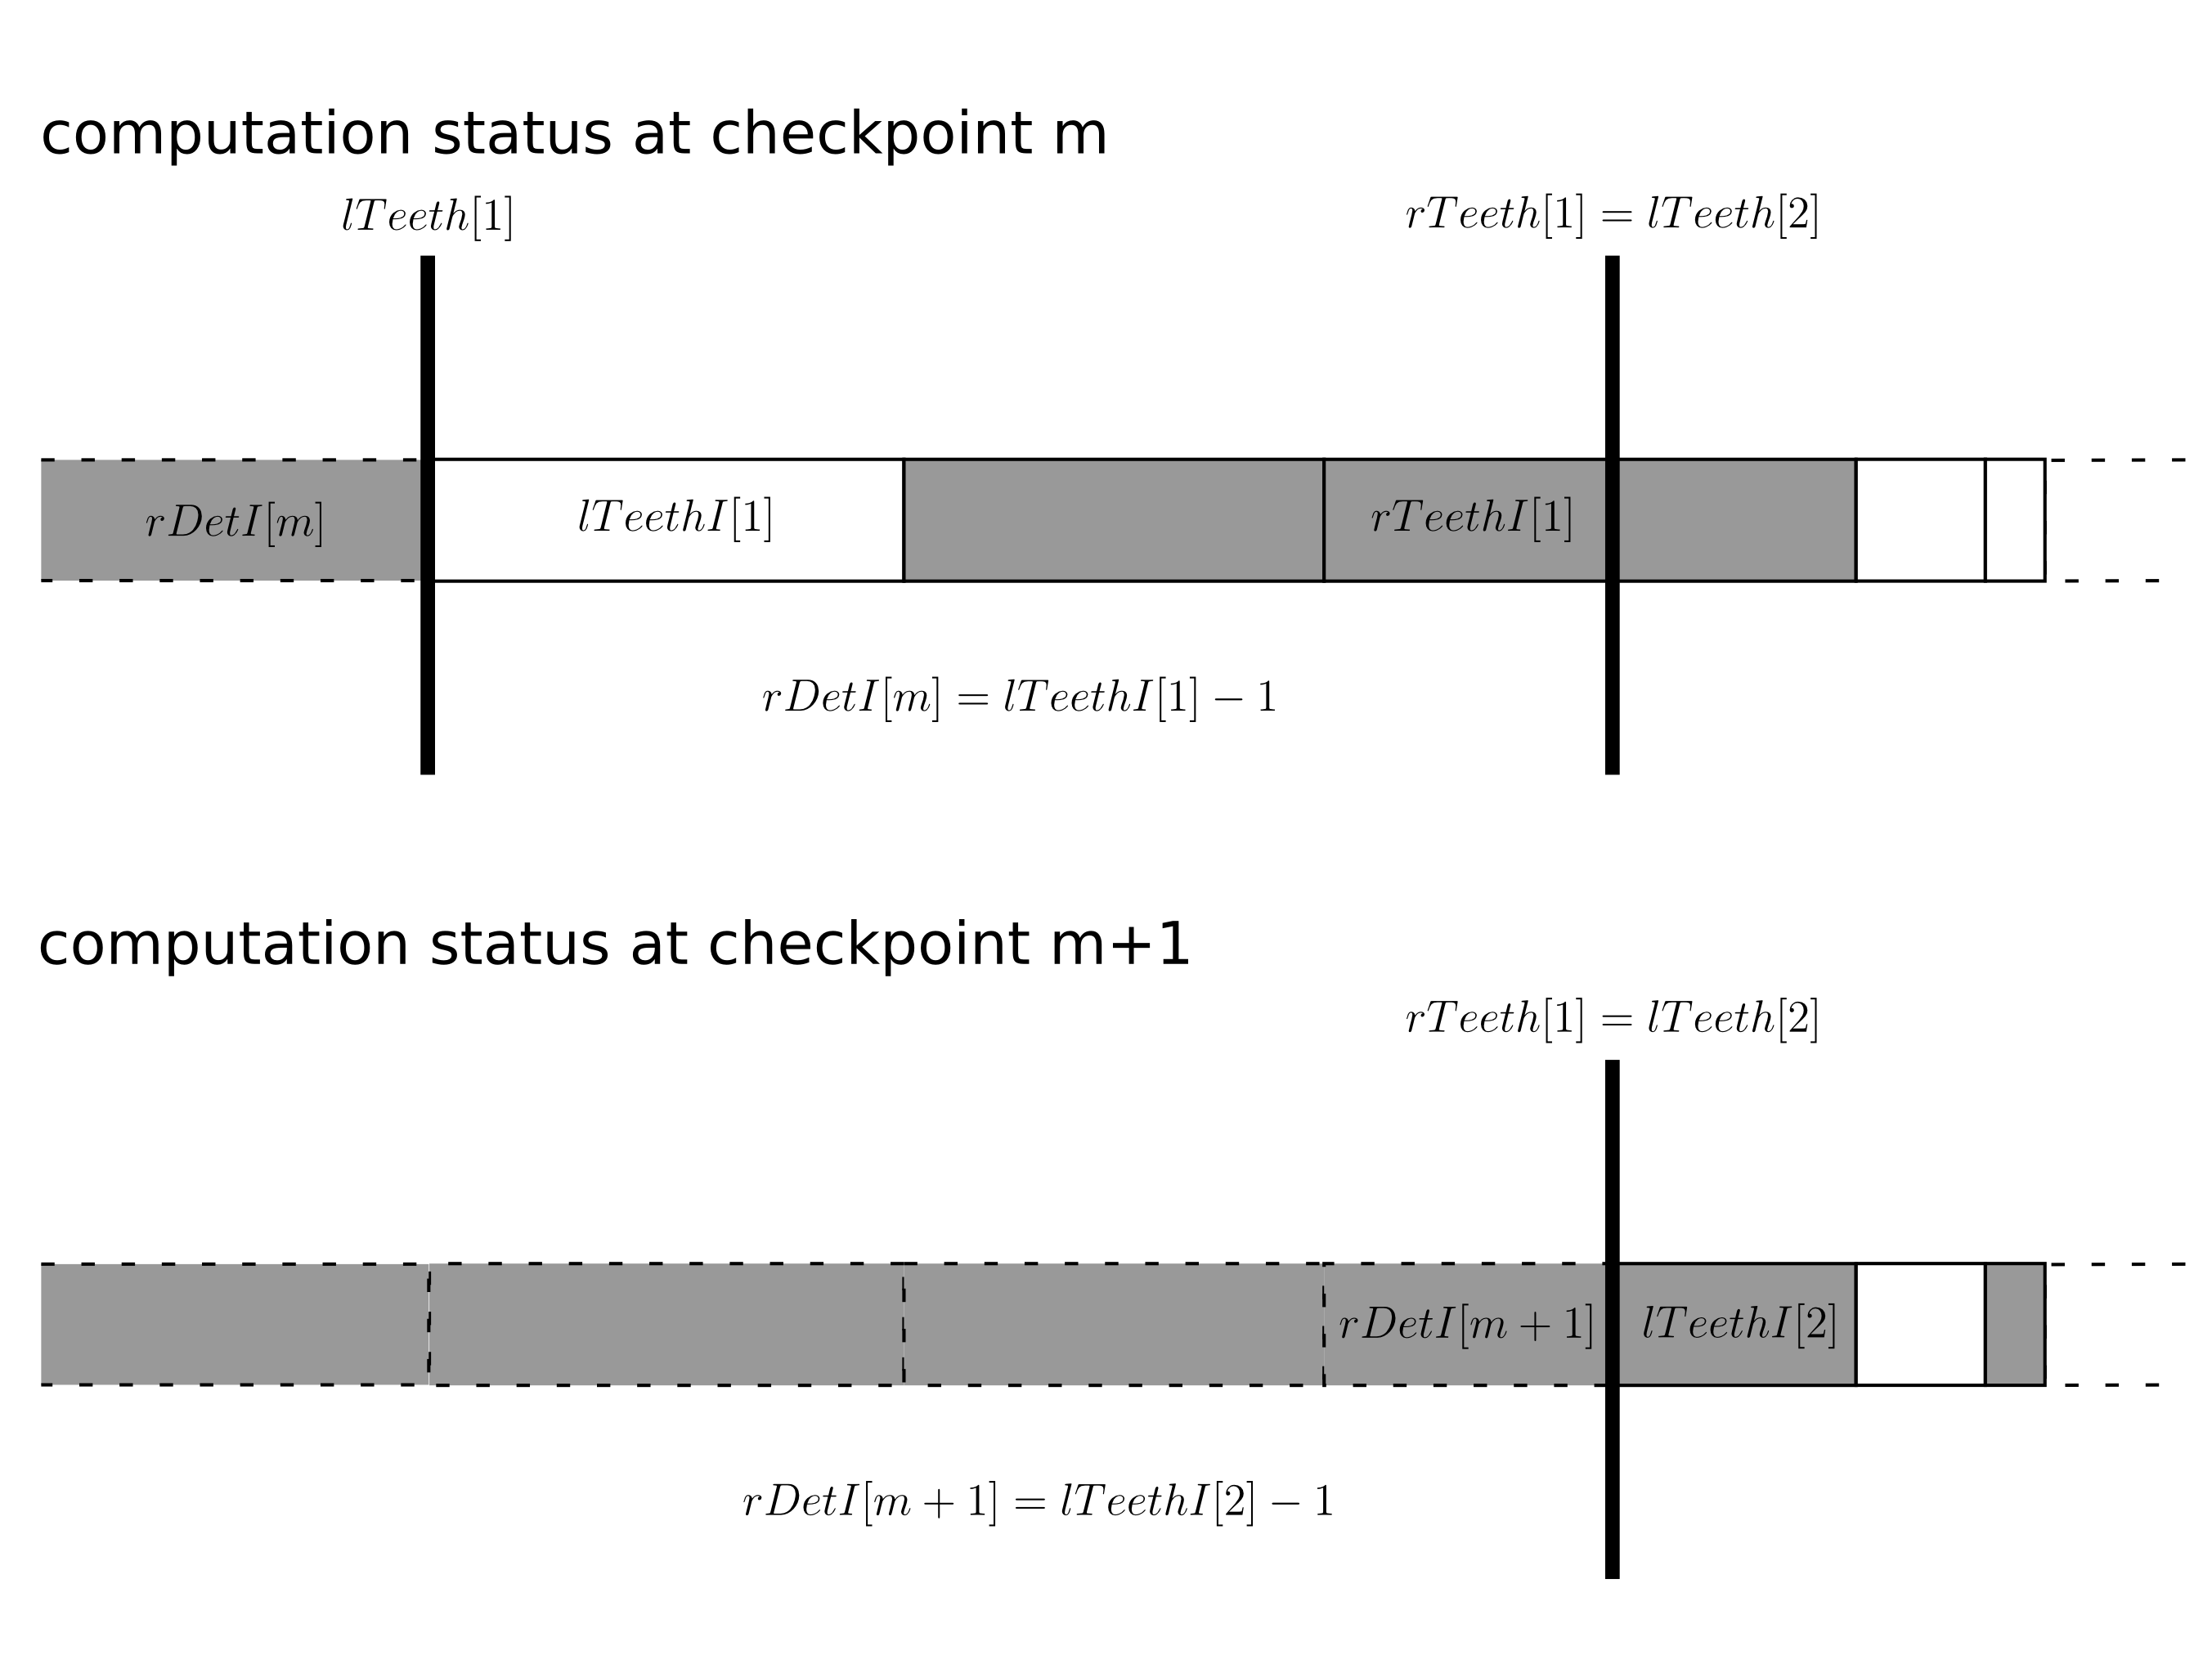
\includegraphics[width=1.00\columnwidth]{figures/matrix_dressing/deterministic_cp}
		\caption{\label{filtering}}
		$rDetI[m]$ gives the index of the last sample of the deterministic part at checkpoint $m$, or $0$ if there is no deterministic part.
		Greyed samples have been computed. Dotted samples are in the deterministic part. Sample $lTeethI[1]$ has been computed between checkpoints $m$ and $m+1$, resulting in tooth $1$ begin fully computed and thus moved into the deterministic part.
	\end{center}
\end{figure}


\end{document}

%%%%%%%%%%%%%%%%%%%%%%%%%%%%%%%%%%% ALGO ARCHIVES
\begin{comment}

\begin{algorithm}
	\label{ADD_COMB}
	\caption{ADD\_COMB}
	\SetKwFunction{FAddComb}{ADD\_COMB}
	\SetKwProg{Fn}{Function}{:}{}
	
	\Fn(\tcc*[h]{Add a comb to the Monte-Carlo by updating $N_{jobs}$, $J$ and $d$}){\FAddComb{$rand, N_{jobs}, J, d,m$}}{
		\KwData{$rand \in [0, 1[$ value associated with the comb to be added}
		\KwData{$N_j$ : number of unique samples computed so far.}
		\KwData{$J_i$ : index of the $i^{th}$ unique sample computed. Will be used as the list of jobs for the actual computation.}
		\KwData{$d_i=TRUE$ if sample $i$ has been computed, $FALSE$ otherwise.}
		\KwData{$m$ : index of current checkpoint}
		
		%$rand \gets RANDOM(0,1)$ \;
		\For{$t=1,N_{teeth}$}{
			$v=lTeeth[t] + rand \times toothSize[t]$ \;
			$i=FIND\_SAMPLE(rand, lTeethI[t], rTeethI[t])$ \;
			$n(curcp, i) += 1$ \;			
			\If{$not\ d_i$}{
				$N_{jobs} \gets N_{jobs} + 1$ \;
				$J_{N_{jobs}} \gets i$ \;
				$d_i \gets TRUE$ \;
			}
		}
	}
\end{algorithm}

\begin{algorithm}
	\caption{PRECOMPUTE\_MONTECARLO}
	\label{PRECOMPUTE_MONTECARLO}
	\tcc*[h]{Computes $J$ the array so that $J_i$ is the $i^{th}$ sample that must be computed to perform the Monte-Carlo computation, and $n[m,i]$ the total number of times sample $i$ has been drawn at checkpoint $m$, regardless of which teeth are in the deterministic part.}
	
	\KwData{$cpthreshold[m]$ is the minimal number of jobs required to reach checkpoint $m$. It's updated to match the end of a comb ( pas clair? )}
	\KwData{$cpthreshold[N_{cpmax}] = N_{gen}$}
		$N_s \gets rDetI[1]$ \;
		$N_j \gets rDetI[1]$ \;
		\For{$i=1,N_j$}{
			$d_i \gets TRUE$ \;
			$J_i \gets i$ \;
		}
		
		$curcp \gets 1$ \;
		$curth \gets 1$ \;
		$U \gets N_j$ \;
		\While{$N_j < N_{gen}$}{
		  $ADD\_COMB($,$RANDOM[0,1]$,$J$, $N_j$, $d$, $n_g)$  \;
		  \While{$U < N_{gen}$}{
		    $U \gets U + 1$ \;
            \If{$not\ d_U$}{
              $d_U \gets TRUE$ \;
              $N_j \gets N_j+1$ \;
              $J_{N_j} \gets U$ \;
              break \;
            }
		  }
		  
		  $N_s \gets N_s + 1$ \;
		  $oldcurth \gets curth$ \;
		  \While{$curth \leq N_{cpmax}$}{
		  	\If{$N_j \leq cpthreshold[curth]$}{
		  		$curth \gets curth + 1$ \;
		  	}
		  }
		  
		  \If{$oldcurth \neq curth$}{

		    $cpthreshold[curcp] \gets N_j$ \;
            $n[curcp,*] = n_g[*]$ \;
            $N[curcp] = N_s$ \;
            $curcp \gets curcp+1$ \;	
		  } 
		}
		$N_{cp} = curcp - 1$ \;
	
\end{algorithm}


\begin{algorithm}
	\caption{COMPUTE\_TEETH}
	\label{COMPUTE_TEETH}
	\SetKwFunction{FMain}{COMPUTE\_TEETH}
	\SetKwProg{Fn}{Function}{:}{}
	
	
	\Fn(\tcc*[h]{Computes teeth thresholds, and $rDetI[1]$ the number or samples in the initial deterministic part}){\FMain{$minDetInTeeth$, $N_{teeth}$}}{
		\KwData{$1 \leq minDetInTeeth \leq N_{det}$}
		\KwData{$N_{teeth} \geq 1$}
		
		$rDetI[1] \gets 0$ \;
		$rcw \gets cw[minDetInTeeth]$ \;
		$lcm \gets 0$ \;
		\While{}{
			$teeth\_width = \frac{1 - lcm}{N_{teeth}}$ \;
			\If{$teeth\_width < rcm - lcm$}{
				break \;
			}
			
			$rDetI[1] \gets rDetI[1] + 1$ \;
			\If{$N_{det} - rDetI[1] < minDetInTeeth \times N_{teeth}$}{
				STOP cannot compute with those parameters \;
			}
			$rcw \gets cw[rDetI[1]+minDetInTeeth]$ \;
			$lcw \gets  cw[rDetI[1]]$\;
		}
		$lTeethI[1] = rDetI[1]+1$ \;
		$lTeeth[1] = lcw$ \;
		$rTeeth[1] = lcw + teeth\_width$ \;
		\For{$i=2,N_{teeth}$}{
			$rTeeth[i] = lcw + teeth\_width \times i$ \;
			$lTeeth[i] = rTeeth[i-1]$ \;
		}
		\tcc{ensure there is no numerical precision error}
		$rTeeth[N_{teeth}] \gets 1$ \;
		
		$t \gets 1$\;
		\For{$i=rDetI[1]+1, N_{det}$}{
			\If{$cw[i] \geq rTeeth[t]$}{
				$rTeethI[t] = i$ \;
				$t \gets t + 1$ \;
			}
		}
		$teethSize[1] = cw[rTeethI[1]] - lcw$ \;
		\For{$t=2,N_{teeth}$}{
			$lTeethI[t] \gets rTeethI[t-1] + 1$ \;
			$toothSize[t] = rTeeth[t] - lTeeth[t]$ \;
		}
	}
\end{algorithm}
\end{comment}
%%%%%%%%%%%%%%%%%%%%%%%%%%%%%%%%%%%
